\item Explain a plan to human agents. Depending on the human expertise on the tasks to be performed, the robot will adapt the explanations, focusing more deeply on tasks that agents do not know how to perform. This idea is supported by research on Intelligent Tutoring Systems \cite{brusilovskiy1994construction}  and on e-learning \cite{brusilovskiy2005}, which  prove the necessity of keeping and updating a model of the learner's knowledge to efficiently teach a task.
	\item Negotiate a plan. Our system has some simple mechanics allowing a human to reject a plan, specifying which parts of it he does not want to perform. The robot will take the human's preference into account when producing a new plan.
	



Some authors have started to investigate this topic in robotics. In \cite{Petit2012}, a human is able to teach new plans to a robot verbally through ``spoken language programming''. \cite{Sorce2015} studies the inverse problem, where the system is able to explain plans to users. 


\section{Human Knowledge and Plan Management}
\label{sec:plan_management-human_knowledge}
\subsection{Representing Human Knowledge in a Task}
Among the topics of this chapter, we will consider different ways to use human knowledge in planning issues. In order to do so, we introduce a new attribute: the human's knowledge of a task, which will be maintained in the Situation Assessment layer. 

This attribute is represented as a tuple $(human, task, parameters, value)$, where $human$ is a string identifying the subject of this attribute, $task$ is the name of the related task, $parameters$ is a list of relevant parameters used to describe knowledge in the task, and $value$ is the level of knowledge in the task. Knowledge values can be assigned from the set $[new, beginner, intermediate, expert]$.  For example, we can represent the fact that Bob knows very well how to fix a wheel to a car with the tuple $(Bob, fix\_wheel, car, expert)$. 

Parameters can be deeply linked to the knowledge of a task. In general, we can divide task parameters in two categories:
\begin{itemize}
\item Class-Link. In some situation, knowledge of a task is not linked to the specific instance of a parameter, but to a whole class. For example, we can imagine that if Bob knows how to paint the living room, he will know how to paint every room in a house. We could represent this attribute as $(Bob, paint, house\_room, expert)$. We can notice that the parameter, in this case, is $house\_room$, representing the class of rooms belonging to a house, and not $living\_room$.
\item Instance-Link. In other cases, instead, knowledge of a task is deeply linked to specific instances of parameters. For example, knowing how to fix the motor of a specific car, would not necessary translate in knowing how to fix the motor of every car.
\end{itemize}

We can also consider some tasks as \textit{common knowledge}, expecting every human to be able to perform them, like, for example, putting ingredients in a bowl. These tasks will be tagged as \textit{common knowledge} and considered as known by any user, no matter the parameters. 

\subsection{Maintaining Human Knowledge in a Task}
%How human update their knowledge
We define four task-knowledge levels for humans, that will lead to different behaviors from the robot.

\begin{itemize}
\item \textit{New}. This value will be used for tasks which have never been performed by the user. If the user observes the task being executed, with an explanation of it, or if he performs it himself, the value will be changed to \textit{beginner}. However if the user observes the task being executed without any explanation, we keep the level as \textit{new} since we consider that he might not have received enough information to link the observed movements to the task.
\item \textit{Beginner}. This value will be used for users who have already achieved the task but may still need explanations to perform it again. If the user successfully performs the task a second time, without asking for explanations, the value is changed to \textit{intermediate}, otherwise it is changed to \textit{new}.
\item \textit{Intermediate}. This value will be used for users who are able to perform the task without guidance. If a \textit{beginner} user successfully performs the task without guidance again, the value is changed to \textit{expert}. In case of failure, it is downgraded to \textit{beginner}.
\item \textit{Expert}. This knowledge level will be used for users who are able to perform the task without guidance and are experienced enough to explain it to a third party. If the user fails in performing the task, he will be downgraded to \textit{intermediate}.
\end{itemize}

Using the knowledge of a task of a human, the system is able to adapt plan generation, explanation, and monitoring to that user.



\subsection{Adapting Plan Generation to Human Knowledge}
\label{subsec:plan_generation-adapting_knowledge}
When interacting with humans, it is important to take into account others' knowledge and capacities when planning. We consider two different policies for our planner: $teaching$, where the planner will look for plans not known to the human, in order to teach him different ways to achieve a task; and \textit{efficiency}, where the robot will try to maximize the number of human tasks known when creating a plan. These ideas were represented as social rules.

To illustrate our planner and the new social rule let us consider an example where a human and a robot have to cook an apple pie. We can consider all the basic actions of this domain (pick, place, cut, etc.) as \textit{common knowledge}, but the human might not know how to perform all the higher level tasks involved. If our policy favors \textit{teaching}, 
the plan should should choose a decomposition with tasks where the human has a low knowledge level. On the other hand, if our policy is \textit{efficiency} the planner should allocate to the human tasks where he is more competent, so that explanations and mistakes are reduced. Using this rule, the robot is able to adapt its plan generation to the knowledge of the user concerning tasks contained in the shared plan. In figure \ref{fig:plan_management-adapting_plan_knowledge} we show an example of plan adaptation for this task with the two policies, using the mental model in table \ref{table:plan_management-apple_pie_human_knowledge}

 
 \begin{table}
\centering
\scriptsize
\renewcommand{\arraystretch}{1.3}
\begin{tabular}{|c|c|}
\hline
Task & Knowledge Level \\ \hline \hline
Cook(ApplePie) & New \\ \hline
PrepareDough(Bowl Mould) & New \\ \hline
PrepareMixture(Bowl Mould) & Intermediate \\ \hline
PrepareFruits(Apple Bowl Mould) & Intermediate \\ \hline
Bake(Mould) & Intermediate \\ 
\hline
\end{tabular}
\caption[Mental model for a human in the Cook Apple
 scenario.]{Mental model for a human in the Cook Apple
 scenario in figure \ref{fig:plan_management-adapting_plan_knowledge} }
 \label{table:plan_management-apple_pie_human_knowledge}    
\end{table}



\begin{figure}[ht!]
 \centering
  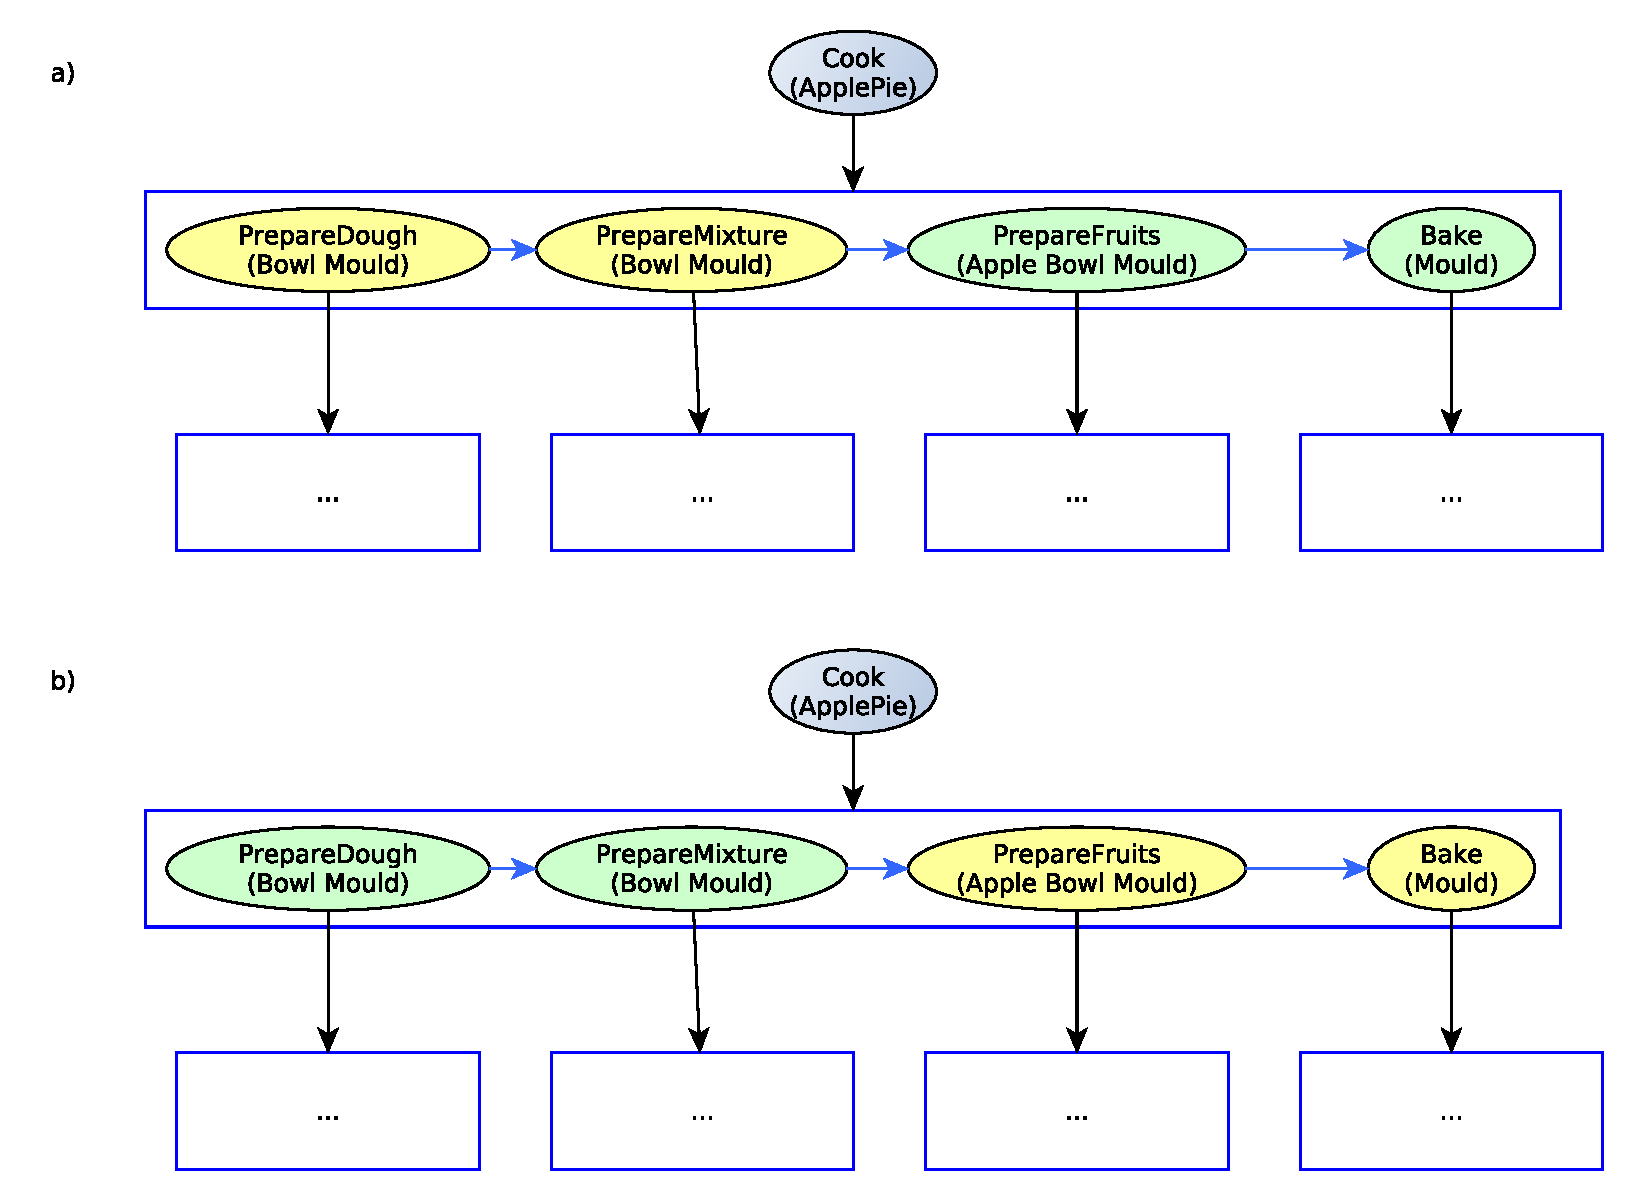
\includegraphics[scale=0.5]{img/plan_management/adapting_plan_knowledge.pdf}
 \caption[Allocation of tasks of a plan to cook an Apple Pie for two agents]{Allocation of tasks of a plan to cook an Apple Pie for two agents, a robot and a human, using the knowledge values in table \ref{table:plan_management-apple_pie_human_knowledge}. A) shows an \textit{efficiency} policy for this task, while b) shows a \textit{teaching} policy for the same task. Blue ellipses represent tasks involving both agents, green ellipses represent tasks assigned to the human, and yellow ellipses tasks assigned to the robot. Each decomposition is grouped in a blue rectangle. Black arrows link a method to its decomposition, while blue arrows represent casual links. Squares with a "..." label represent decompositions that are not shown in this picture.}
 \label{fig:plan_management-adapting_plan_knowledge}
 \end{figure}



To properly compute the cost of a plan, the planner will also upgrade accordingly the knowledge of a task once it is added to the plan. This allows the \textit{efficiency} policy to prefer plans with repetitive decompositions, that are assigned to the same user, over plans with more variable decomposition, where repetitive tasks are assigned to different agents.

The planner can receive information produced from a dialog system that allows to negotiate plans, as explained in section \ref{sec:plan_management-negotiation}. Using this system, the preference and abilities of users are recorded in the Situation Assessment layer. 
If a user is not able to perform a certain task, the planner will never chose this action for him. If he user prefers to perform, or not to perform, a specific task, the planner will update the cost functions accordingly with a reward or penality to assign that task to him.


\subsection{Plan Presentation}
Before executing the plan, the robot will present the goal and the proposed allocation of high-level tasks to give a global view of the chosen strategy. Standard natural language generation is used, as shown in table \ref{table:plan_management-pie-present}. 
In some situations, the plan will be too long to explain it at the same time to a user, which could then be confused or annoyed. For this reason, when presenting the plan, the robot will verbalize only the first $N$  highest level tasks. We have chosen $N$=$3$ based on our own experience during tests with the system, but we can imagine to adapt it to the complexity of the domain, or even to specific users. The robot will present the first steps of the plan, perform a negotiation phase, and then execute them. Once these tasks have been executed, the robot will repeat the present/negotiate/execute process until the plan is completed or aborted.
 
 \begin{table}
 %\vspace{-10pt}
\centering
\scriptsize
\renewcommand{\arraystretch}{1.3}
\begin{tabular}{c|c}
   agents(root) $+$ have\_to $+$ root  & "We have to cook an apple pie." \\
   \hline
   introduce\_presentation & "I will tell you the steps." \\
   \hline
   agents(child[0]) $+$ first $+$ child[0] & "You will first fetch the ingredients," \\
   \hline
   then $+$ agents(child[1]) $+$  child[1] & "Then I will assemble the apple pie," \\
   \hline
   finally $+$ agents(child[2]) $+$  child[2] & "Finally, you will bake \\
   & the apple pie in the oven." \\
\end{tabular}
\caption[Presentation of a plan to cook an apple pie]{Presentation of a plan to cook an apple pie. Root is the root of the HTN tree and child is a list with its children.}
 \label{table:plan_management-pie-present}    
\end{table}

\section{Plan Negotiation}
\label{sec:plan_management-negotiation}
Once the robot has presented the plan to his collaborators, it can start a negotiation phase. 

We introduce a simple negotiation algorithm, that starts with the robot asking humans for approval of the plan, inquiring what is wrong in case of disagreement. We handle two different human requests. First, the user can express his preferences, either to perform a task previously assigned to the robot or to not perform a task assigned to him. The other possibility is to inform the robot that the user cannot perform an action. The system will store these information and try to find a new plan, taking them into account, before starting a new explanation and negotiation phase.


\subsection{Sequential Adaptive Plan Management Algorithm}
\label{subsec:plan_management-sequential_plan_management}
We start this subsection by showing our sequential plan management algorithm, and then we explain it.

%\begin{algorithm}
\begin{algorithmic}[1]
\For{n$:=$nodes.start to n$:=$nodes.end}
	\If{$agents$(n) = \{robot\}}\label{alg:onlyRobotStart}
    	\If{$children(n) \neq \emptyset$ $\wedge$ $user\_kn(n)$ = new\par
        \hskip\algorithmicindent $\wedge$ $teachPolicy$}
        	\State $execute\_tree(children(n))$
            \State $user\_kn(n) :=$ beginner
        \Else
         	\State $execute(n)$
        \EndIf\label{alg:onlyRobotEnd}
    \ElsIf{$user\_kn(n)$ = new}\label{alg:newStart}
     	\State $explain(n)$
        \If{$children(n)$ $\neq \emptyset$}
          	\State $execute\_tree(children(n))$
            \State $user\_kn(n)$ $:=$ beginner
        \Else
         	\State $monitor(n)$
        \EndIf\label{alg:newEnd}
    \ElsIf{$user\_kn(n)$ = beginner}\label{alg:beginnerStart}
      	\If{$propose\_explain(n)$}
          	\State $user\_kn(n)$ $:=$ new
            \State $(\dots)$ \Comment{Same process as new}
        \Else
          	\State $monitor(n)$
        \EndIf\label{alg:beginnerEnd}
    \ElsIf{$user\_kn(n)$ = intermediate\par
    \hskip\algorithmicindent $\vee$ $user\_kn(n)$ = expert}\label{alg:interStart}
      	\State $monitor(n)$
    \EndIf\label{alg:interEnd}
\EndFor
\end{algorithmic}
%\caption{$execute\_tree(n)$}

%\end{algorithm}

\begin{itemize}
\item \textit{$execute\_tree(n)$} is the main plan management function. The function receives as argument \textit{$nodes$}, a list of nodes initially filled with the root's children.
\item \textit{$teachPolicy$} is a boolean that defines if we are in teaching or efficient mode.
\item \textit{$agents(n)$} returns the agents involved in the node \textit{n}.
\item \textit{$verbalize(n)$} will verbalize the current task, using the node context to present it (e.g. using sequential relations such as first, then or finally according to the node position in the list).
\item \textit{$user\_kn(n)$} returns the knowledge level of the user concerning the task \textit{n}.
\item \textit{$propose\_explain(n)$} will lead the robot to propose an explanation for the current task. If the user accepts the explanation it will return true, and otherwise false.
\item \textit{$explain(n)$} launches a procedure to explain the current task to the user. This procedure could be implemented as a script to launch a video, an explanation speech or even to ask an expert to explain the task.
\item \textit{$monitor(n)$} starts monitoring the proper execution of the current node. If the request returns a success, the function will upgrade the user's knowledge and the \textit{$execute\_tree$} function will continue. In case of failure, the function will downgrade the user's knowledge, exit the \textit{$execute\_tree$} function, and return a failure that will result in a replan request and a new execution if a plan is found.
\item \textit{$execute(n)$} works in a similar way to the monitor but sends a request to execute the node by the robot.
\end{itemize}
 
\subsection{Explanation of the sequential plan management algorithm}
This plan management algorithm is based on the structured plan tree computed by the task planner, and on the tasks' knowledge values in the user models. We explore this tree with a pre-order strategy. The algorithm will analyze each node, with several possible outcomes:

\subsubsection{Only the robot is involved (lines ~\ref{alg:onlyRobotStart}-~\ref{alg:onlyRobotEnd})}
If the robot is the only agent in charge of the current node, the collaborator has a knowledge level equal to \textit{new} for the current task,
and the chosen policy for the interaction is teaching, then the robot will execute the subtasks in ``demonstration mode'', meaning that it will verbalize each child task before performing it.

Once the task have been executed, the robot updates the human's knowledge on the current node to \textit{beginner}. The same process will be applied to the tasks' children.  Using this process, the robot will verbalize each (and only) task that needs to be learned by the collaborator.

If the robot is in charge, but the human collaborator's knowledge on the task is different from \textit{new}, or the current policy is efficiency, the robot will verbalize only the high-level task it performs.

If the human is involved in the current node, the robot's behavior will depend on the human's knowledge level for the task, since the human might need explanations.  Explaining a task could be done in several ways: showing a video, asking an expert to explain the it or simply verbally guiding the user, step by step.
\subsubsection{The collaborator's knowledge level on the task is \textit{new} (lines~\ref{alg:newStart}-~\ref{alg:newEnd})}
If the human has a level $new$ for the current task, we explain it.
When verbally guiding the user, if the current node has only one child, we  go deeper in the tree and apply again the corresponding behavior according to the knowledge level. If the current node is actually an operator (a leaf), the system monitors the current action execution. In case of success, the knowledge level for the task is upgraded to \textit{beginner}.

% if beginner
\subsubsection{The collaborator's knowledge level on the task is \textit{beginner} (lines ~\ref{alg:beginnerStart}-~\ref{alg:beginnerEnd})}
 If the human has a level \textit{beginner} for the current task, we ask if he needs explanations. If so, we downgrade his knowledge level to $new$ on the current task and apply the same process as the previous paragraph. If the user refuses explanations, we simply monitor the execution of the current node. In case of success, the knowledge level for the current task is upgraded to \textit{intermediate}. This knowledge level will also be used as default. This way, when the robot does not know the knowledge level of an agent concerning a task, it will just ask him if he needs an explanation and adapt its behavior accordingly.

% if intermediate
\subsubsection{The collaborator's knowledge level on the task is \textit{intermediate} (lines~\ref{alg:interStart}-~\ref{alg:interEnd})}
 If the human has a level \textit{intermediate} for the current task, we verbalize it without proposing explanations, since he has already  succeeded with the plan at least once without help. Also, we do not go deeper in the tree and directly monitor the current task. If the user  fails, we downgrade his knowledge to \textit{beginner}, otherwise we upgrade it to \textit{expert}.

% if expert
\subsubsection{The collaborator's knowledge level on the task is \textit{expert} (lines~\ref{alg:interStart}-~\ref{alg:interEnd})}
 In case of an \textit{expert} knowledge level on the current task, we  proceed as for the previous knowledge level, downgrading the level to \textit{intermediate} if the user makes a mistake and keeping the \textit{expert} level if he performs the task as expected.



\subsubsection{Replanning}
When the plan manager reports a failure, the system needs to look for a new plan. If possible, we would like to create a plan which contains the same high-level task allocation. Sometimes, when the Plan Manager fails, there is no need to completely change the plan. Instead, it might be sufficient to repair only a part of it. For example, we can imagine a scenario where a human might execute task $t_1$ using resource $r_1$ or $r_2$. Perhaps the robot computed a plan where the human will use resource $r_1$, while itself will use $r_2$ to achieve another task.

If the human does not follow this plan, and uses $r_2$ to compute its task,  it might be faster to just repair the plan, looking for a solution where the task allocation is the same, but the robot uses $r_1$ instead to achieve its task. This way, we avoid starting a new explanation\textbackslash negotiation phase, which could look useless and not natural to the human collaborator.

%  We deal with this issue in different ways in HATP and HAPP.

In HATP, we introduce a new cost rule. When presenting a plan, we record which nodes have been presented and assigned to each agent. While planning, we penalize plans with a different task allocation. This way, the planner will prefer to use the same task allocation, but will change it if needed, for example because, using the previous task allocation, the goal is no longer achievable.

%In HAPP, we can just perform a partial replan, by interrogating the currently active MMODP.  




\section{Experiments and Discussion}
\label{sec:plan_management-experiments}
In this section, we present a set of experiments which where performed to evaluate the performance of the Plan Explanation and Sequential Adaptive Plan Management systems.

 \subsection{Experiment}
 \label{sec:plan_management-experiment}
To test our system, we have chosen a scenario where a human is trying to prepare two desserts, an apple pie and a banana pie, without knowing their recipes. The robot's goal is guiding and assisting the user, as shown in figure \ref{fig:plan_management-scenario}. 

\begin{figure}[ht!]

 \centering
 \begin{tabular}{cc}
  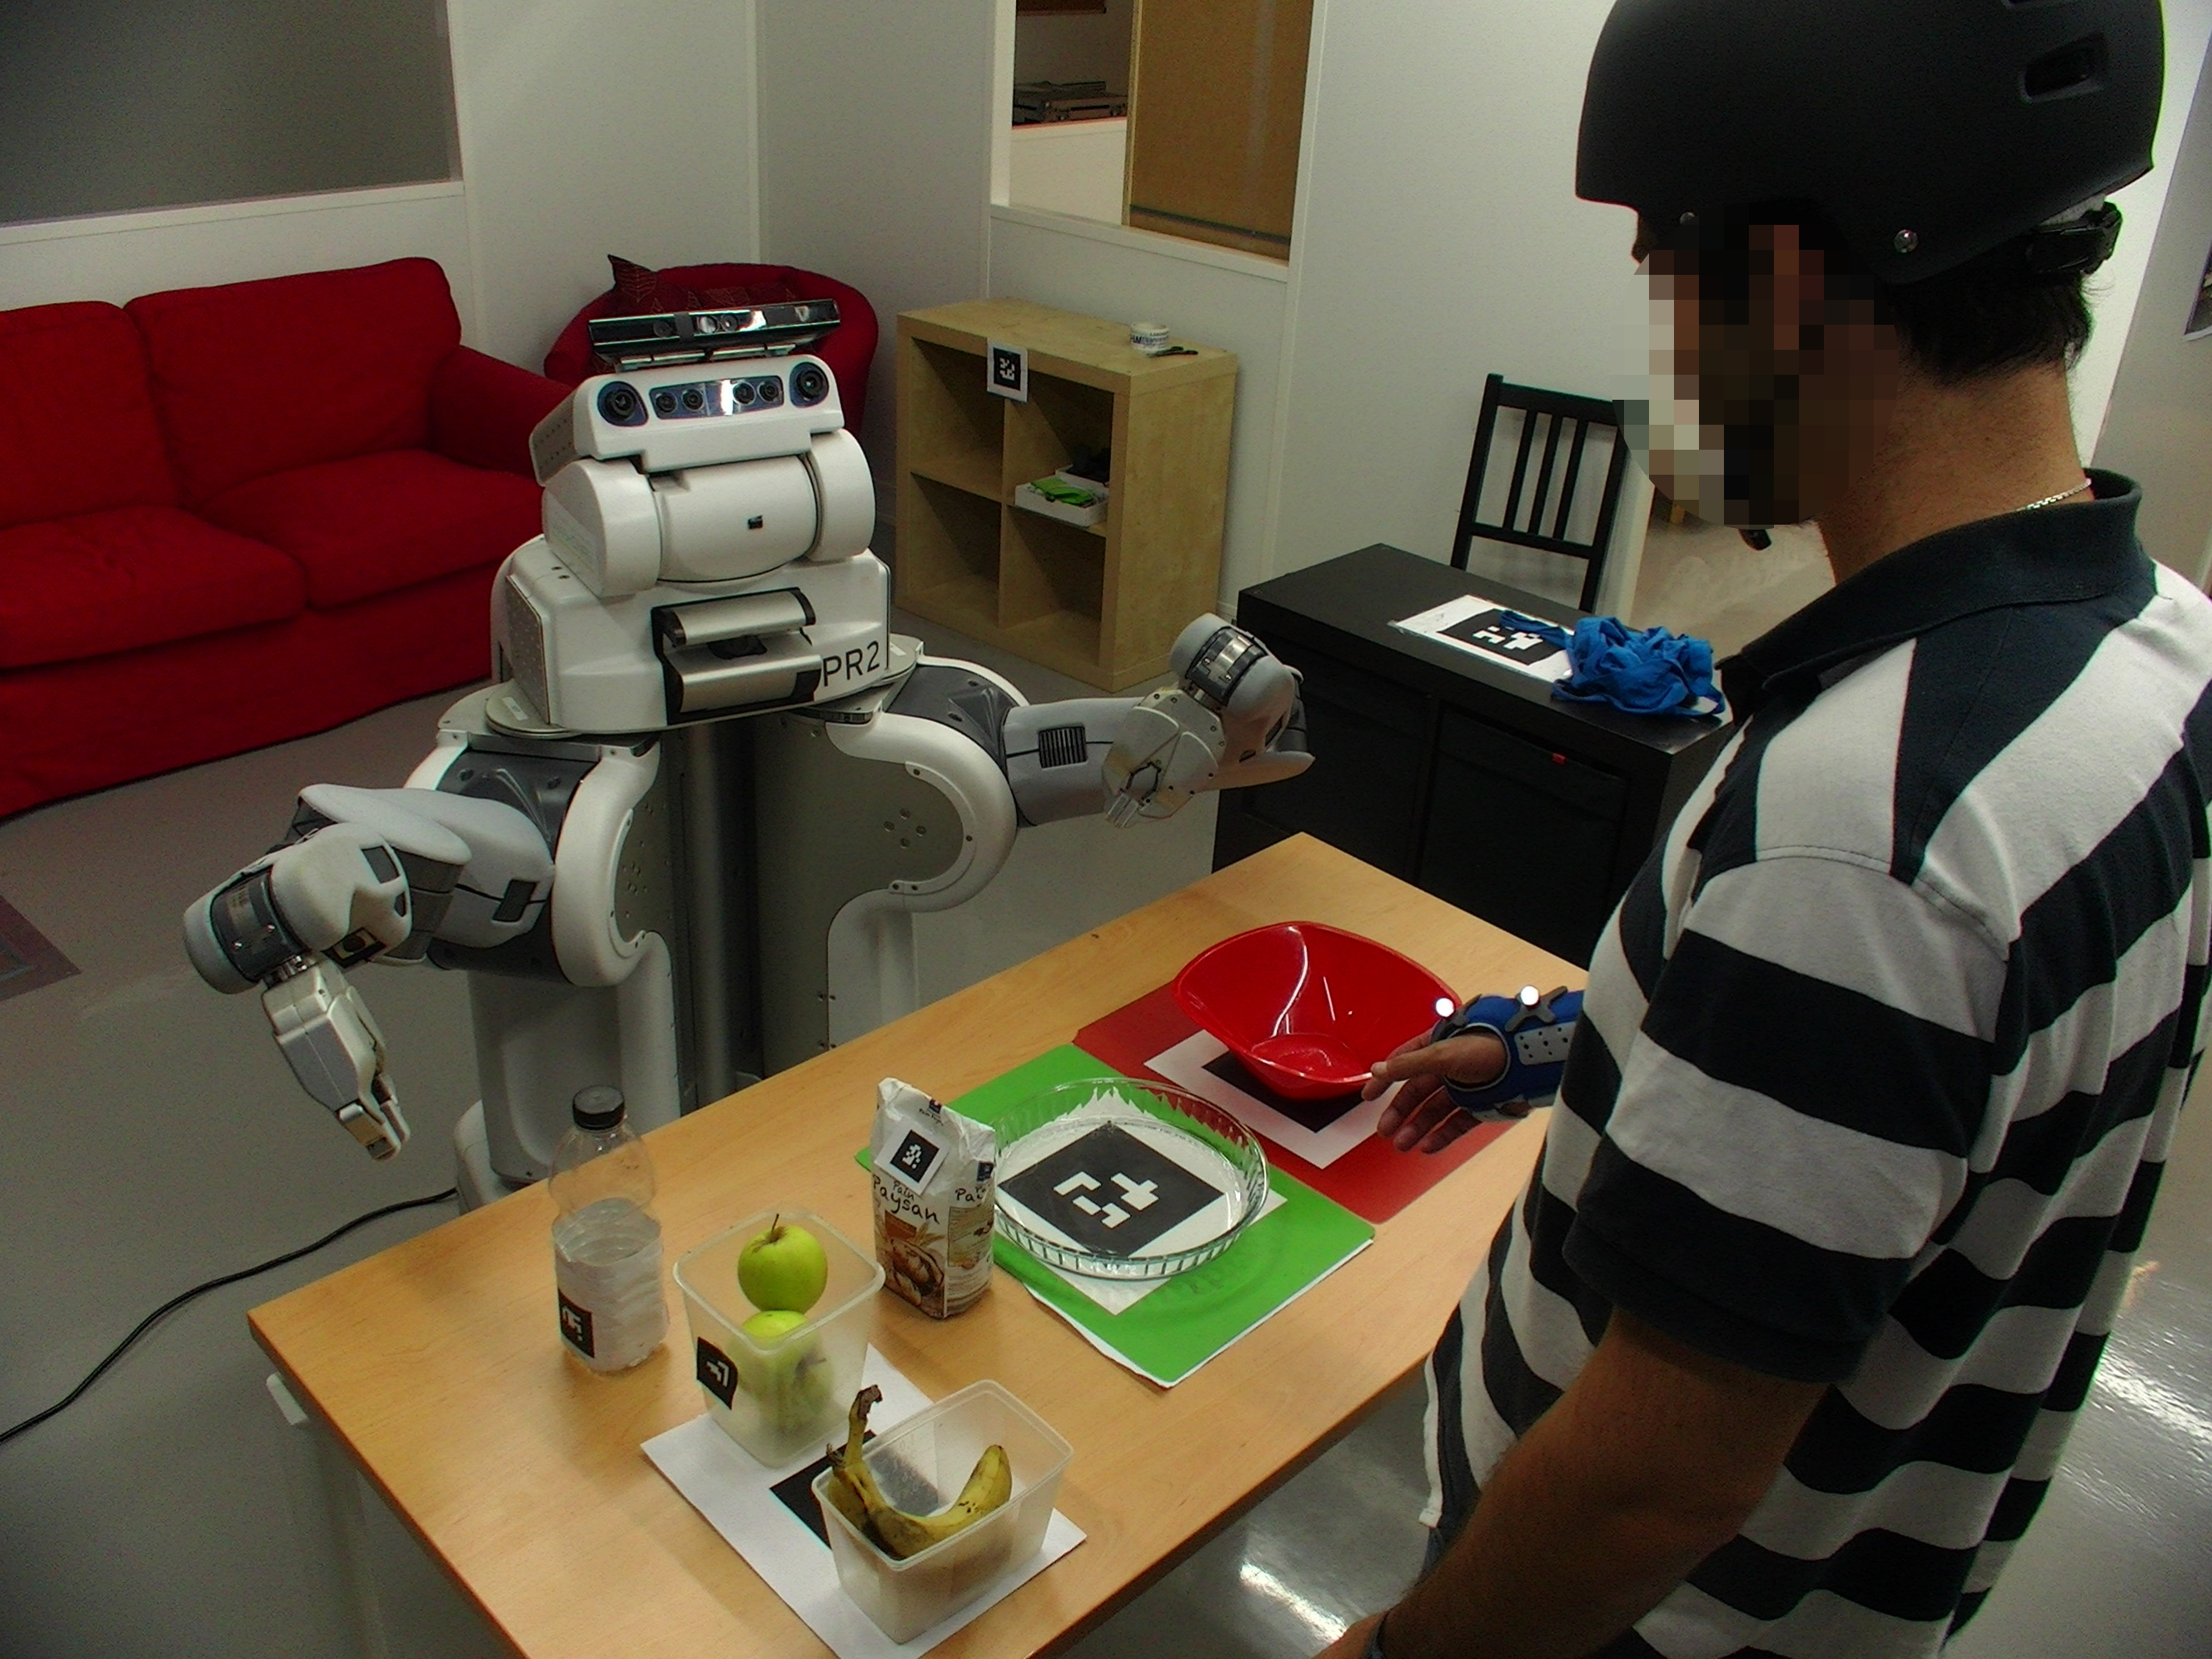
\includegraphics[width=0.29\textwidth]{img/plan_management/scenario.JPG}
 \end{tabular}
 \caption{Illustration of the cooking pies scenario}
 \label{fig:plan_management-scenario}
 \end{figure}

We created a domaint to represent this scenario, and tested it using the previously explained \textit{efficiency policy} and HATP as task planner. To process of cooking an apple pie involves five main tasks. We imagine that, in our set-up, the robot is not able to execute the \textit{PrepareDough} and \textit{PrepareFruits} tasks, since it can not reach the needed ingredients. HATP produces a plan, allocating the tasks as follows:

\begin{figure*}[ht!]
 \centering
 \begin{tabular}{cc}
  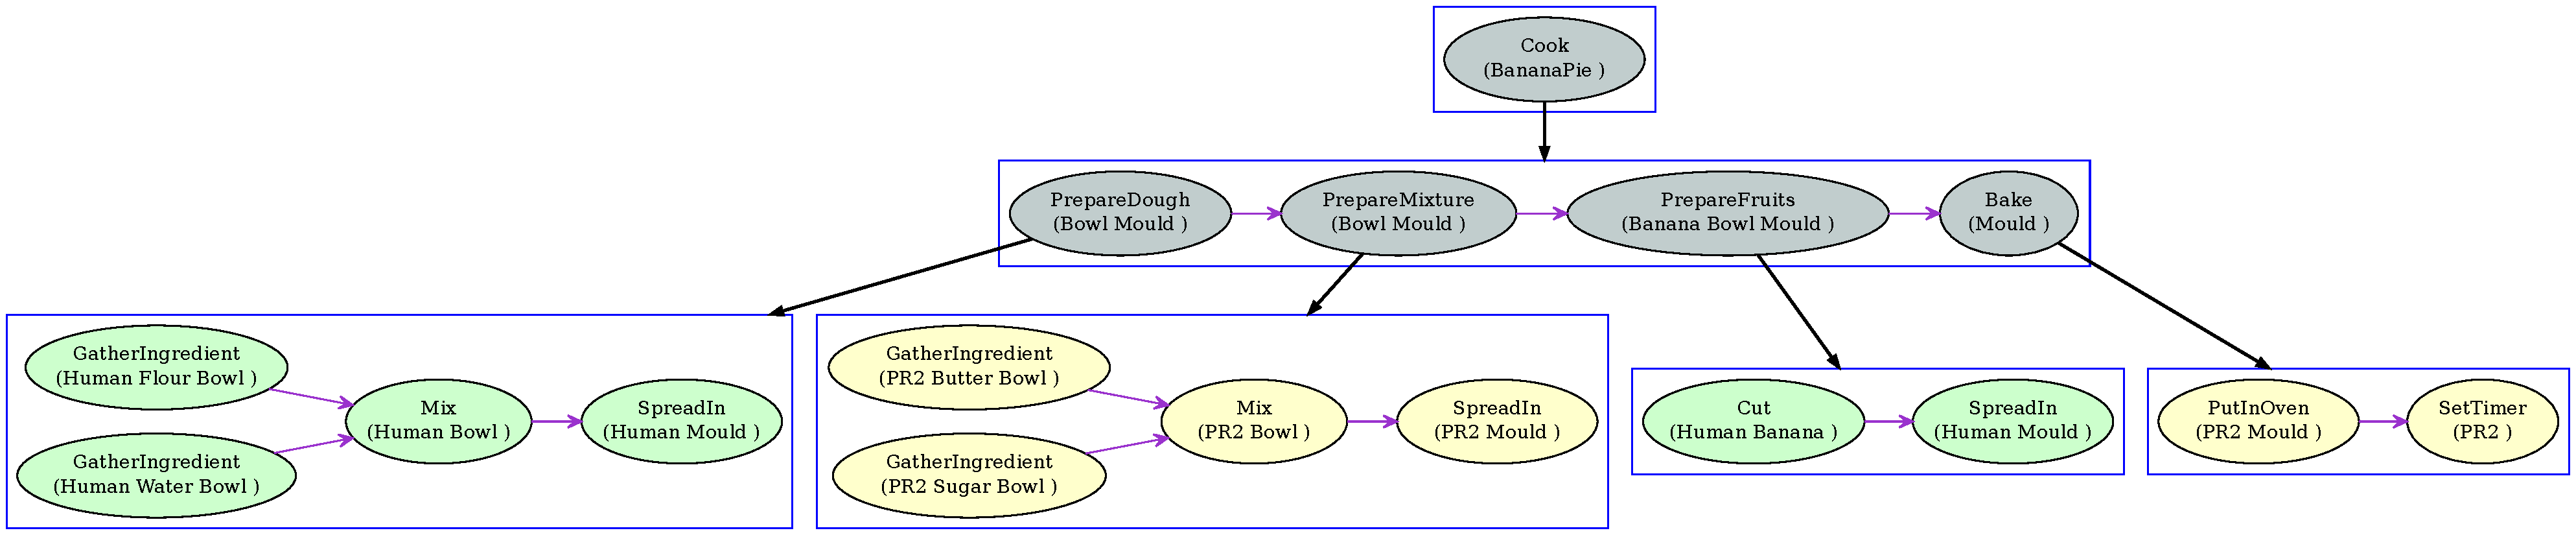
\includegraphics[width=0.99\textwidth]{img/plan_management/bananaPie.pdf}
 \end{tabular}
   \vspace{-8pt}
 \caption{Shared plan and associated HTN generated to collaboratively make a banana pie.}
 \label{fig:plan_management-bananaPlan}
   \vspace{-22pt}
 \end{figure*}
 

\begin{enumerate}
\item The human will prepare the dough, kneading it and putting it in the mould.
\item The robot will prepare a mixture with butter and sugar, putting the ingredients in the mould.
\item The human will then prepare the required fruits, cutting them and adding them to the mixture..
\item Then, the human will prepare the dough for the top of the pie.
\item Finally, the robot will bake the pie, by putting it into the oven and setting a timer.
\end{enumerate} 

After completing task 1, the human's knowledge on how to prepare the dough will be improved. Consequently, during the execution of task 4, the robot will ask the user if he needs help to prepare the second dough. We imagine he answers ``no". The robot does not explain the task  and the system will upgrade the human's knowledge level for the \textit{PrepareDough} task to  \textit{intermediate}, after he completes. The human's knowledge of task 3, \textit{PrepareFruit}, will be represented as \textit{$<$human1, PrepareFruits, [fruit], VALUE$>$}. We consider the parameter of this task as \textit{class-link} , since the process will be the same for any fruit (cutting and putting in the mould). This way we use, as parameter, the class \textit{fruit} instead of the actual instances used in the task, \textit{apple} or \textit{banana}.

After cooking the first pie, the robot generates a plan to cook the banana pie. This time, we set the environment in order to allow  each agent to perform all the tasks. Preparing a banana pie is a similar process to the apple pie. The parameter will, of course, be differents, involving bananas and not apple. Also, the banana pie does not have a second dough on its top, and it has a different baking time from the apple pie. The plan generated is presented in figure \ref{fig:plan_management-bananaPlan}. We can observe that the planner took into account the experience acquired by the human when preparing the apple pie, by assigning him the tasks (\textit{PrepareDough} and \textit{PrepareFruits}). During execution, since the user has an \textit{intermediate} knowledge level on \textit{PrepareDough}, the robot will not explain it. When the human is about to execute \textit{PrepareFruits}, the robot will propose to explain him the task, since he only performed it once, and has a \textit{beginner} knowledge level on it.


\subsection{User Study}
We have conducted a comparative user study in order to have a first evaluation of our system's adaptability by users. Two groups of users were asked to participate in the two-pies scenario. The first group interacted with a simulated robot equipped with a basic system (BS). BS has the same behavior as our system, excluding the agent knowledge awareness mechanisms. The second group interacted with another system, which we will refer to as knowledge system (KS), and exhibits similar characterstics to the presented system.

The hypothesis of our study is that, on average, users will express a preference on KS over BS. More formally, we set our null $H_0$ and alternative $H_A$ hypotheses as follows:
\begin{itemize}
\item $H_0$: $\mu_{KS}-\mu_{BS}==0$ 
\item $H_A$: $\mu_{KS}-\mu_{BS}!=0$  
\end{itemize}


In both system, we will use the same task allocation presented in subsection \ref{sec:plan_management-experiment} to achieve the apple pie cooking example. Once the have cooked the first dessert, the robot generates a plan to cook the banana pie. 
In KS,  the robot favors a task distribution for the banana pie where the human performs tasks he has already executed in the previous scenario (preparing dough and fruits).
In BS, we imagine that the robot could allocate the tasks differently, asking the human to prepare the mixture instead of the dough.

Two groups of 19 participants, from 18 to 60, interacted with each system in an online user study\footnote{User study for KS http://goo.gl/forms/qvbtu4vcFW, and BS http://goo.gl/forms/ZSvGcCi5le}, where we presented pictures of the task state and recordings of the robot's speech, in French, for each step of the interaction (as shown in figure~\ref{fig:plan_management-user_study}).
At some steps, the user could choose the action to perform, allowing him to execute a wrong action, leading to a replan from the robot. For simplicity, the replan just corrected the wrong action, before resuming the previous plan. Also, since the focus of this study is only on the capacity of our system to adapt to users' knowledge, we did not allow a negotiation process.
At the end of the simulated interaction, we have asked the same questions to both groups, concerning the adaptability of the system and the robot partner itself. 
The users gave marks along a Likert scale from one (disagree) to five (agree) to express their agreement with several statements (as shown in figure \ref{fig:plan_management-user_study}).

\begin{figure}[ht!]
 \centering
 \begin{tabular}{cc}
  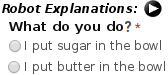
\includegraphics[width=0.24\textwidth]{img/plan_management/ustudy9.png} &
  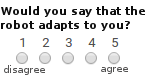
\includegraphics[width=0.19\textwidth]{img/plan_management/ustudy11.png}
 \end{tabular} 
 \caption[User studies on plan adaptation]{\textit{Left}: The user listens to recorded robot explanation and chooses the action to take. \textit{Right}: At the end, the user evaluates the interaction using a Likert scale.}
 \label{fig:plan_management-user_study}
 \end{figure}

\subsection{Results}

We collected the answers from each form, and computed the mean, along with the standard deviation and p-value to evaluate the system. The p-value was computed using a t-distribution with 18 degrees of freedom and evaluated using a significance value $\alpha=0.05$.
%We compare below the results for each system. 
Figure~\ref{fig:plan_management-results} summarizes the results. Comparing users' answers, we can see that user appreciated the capacity of the system to explain the plan while  adaptation on their knowledge, with a mean of 3.74 for KS against 2.05 for BS. The users interacting with KS globally noticed that the task distribution took their knowledge into account, by giving a mean rating of 3.42 for KS and 2.58 for BS. The last question concerned the freedom to choose how to perform the task. In this case, the calculated mean was 2.58 for KS and 1.89 for BS. In all these cases, the p-value was lower than the $\alpha$. 

With KS, the users attributed a mean of 3.11 for the global adaptability of the system against 1.89 for the basic one.
We also asked how the robot partner was perceived. While in KS the robot is not perceived as more verbose (2.53 for KS against 2.47 for BS), people found the interaction slightly more natural (2.74 against 2.42) and the robot appeared smarter (2.79 against 2.26). Even if these last two results look favorable, since their p-value is higher than $\alpha$  we do not have enough evidence to prove a difference between the two systems. We believe that other aspects might have been taken into account by the users, such as the speech itself, which conditioned their perception on the naturalness of the interaction. Improving the robot's verbalization process with a synonym dictionary could be a first step to get more significant results.



 \begin{figure}[ht!]
 \centering
 \begin{tabular}{cc}
  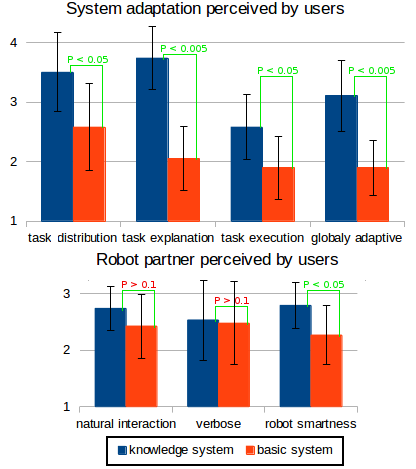
\includegraphics[width=0.45\textwidth]{img/plan_management/respvalue3.png}
 \end{tabular}
 \caption[Average users' rating of the interaction on several criteria]{Average users' rating of the interaction on several criteria. Blue for KS and red for BS.}
 \label{fig:plan_management-results}
 \end{figure}

This study sheds light on how users were able to perceive the robot adaptation to their knowledge concerning task distribution, task explanation and monitoring. In addition, the robot partner was perceived as smarter and the interaction seemed a bit more natural to the users. However, these first results need to be confirmed with study on a larger population. Also, as the scenario was simulated, results on a real robot might differ.
In both studies, we asked the participants how the system could be improved. Several users suggested they would like to be able to choose which action to perform, showing the importance of negotiation. A user suggested he would like to be informed about the progress of the task from time to time. Other comments concerned suggestions about the robot's speech capacities, like its voice voice, its intonation, and the chosen words. These aspects were not the aim of our  experiment but are indeed an important part of the interaction process. 

%


